\documentclass{article}
\pagenumbering{arabic}
\usepackage{graphicx,amsmath,amssymb,bm,tikz}
\usetikzlibrary{calc,patterns,decorations.pathmorphing,decorations.markings}
\usepackage{xfrac}
\usepackage{array}
\newcolumntype{P}[1]{>{\centering\arraybackslash}p{#1}}
\newcolumntype{M}[1]{>{\centering\arraybackslash}m{#1}}
\usepackage[utf8]{inputenc}
\usepackage{hyperref}
% Format fref 
\usepackage[plain,english]{fancyref}
\usepackage[margin=1in]{geometry} 
\fancyrefaddcaptions{english}{\renewcommand*{\frefeqname}{Eq.}}
% Figure Packages
\usepackage[outercaption]{sidecap}
\usepackage[export]{adjustbox}
\usepackage{graphicx}
\usepackage{caption}
\usepackage{wrapfig}
\usepackage{float}
\usepackage{algorithm, algorithmic, amsfonts,amsmath,amssymb,amsthm, color,comment,enumitem, environ, fancyhdr,   graphicx, mathtools, wasysym}
\pagestyle{fancy}
\setlength{\headheight}{22.55pt}
\newenvironment{problem}[2][Problem]{\begin{trivlist}
\item[\hskip \labelsep {\bfseries #1}\hskip \labelsep {\bfseries #2.}]}{\end{trivlist}}
\newenvironment{sol}
    {\emph{Solution:}
    }
    {
    \qed
    }
\specialcomment{com}{ \color{blue} \textbf{Comment:} }{\color{black}} %for instructor comments while grading
\NewEnviron{probscore}{\marginpar{ \color{blue} \tiny Problem Score: \BODY \color{black} }}
%%%%%%%%%%%%%%%%%%%%%%%%%%%%%%%%%%%%%%%%%%%%%%%%%%%%%%%%%%%%%%%%%%%%%%%%%%%%%%%%%





%%%%%%%%%%%%%%%%%%%%%%%%%%%%%%%%%%%%%%%%%%%%%
%Fill in the appropriate information below
\lhead{Bulldog AeroAcoustics, LLC \\ Daniel Agramonte}  %replace with your name
\rhead{MCHE 6390 \\ Project 2 - Final Report} %replace XYZ with the homework course number, semester (e.g. ``Spring 2019"), and assignment number.
%%%%%%%%%%%%%%%%%%%%%%%%%%%%%%%%%%%%%%%%%%%%%



% Table stuff
\usepackage{multirow}
%\usepackage{floatrow}
%	\floatsetup[table]{capposition=top}%puts table caption above
% Change \subsection title characteristics
    \usepackage[parfill]{parskip}   % forces parskip to not affect headings
    \usepackage{enumitem}           % used for editing itemize environment
    \usepackage{titlesec}
        \titleformat*{\section}{\Large\bfseries\titlerule\vspace{0.5em}}
% Quote blocks
    \usepackage{csquotes} % use environment 'displayquote'
% Misc document settings
    \title{\Huge MCHE 6390 Project 2} 
    \author{Daniel Agramonte \\ Bulldog AeroAcoustics, LLC.}
    \date{12.17.20}
    \setlength{\parindent}{0pt}
    \setlength{\parskip}{1em}
    \setlist{nosep, itemsep=0pt, parsep=0pt}
% Misc vocab commands
    \newcommand{\msalg}{{\fontfamily{cmtt}\selectfont ms83}}
    \newcommand{\lsq}{\emph{lsqnonlin}}
    \newcommand{\fmin}{{\fontfamily{cmtt}\selectfont fmincon}}
    \newcommand{\atand}{{\fontfamily{cmtt}\selectfont atan2d}}
\DeclareMathOperator\supp{supp}
\DeclareMathOperator*{\argmax}{arg\,max}
%
% MATLAB packages
%
\usepackage[framed,numbered]{matlab-prettifier}
\usepackage{textcomp}
\usepackage{listings}
%
% Matrix Spacing
%
\makeatletter
\renewcommand*\env@matrix[1][\arraystretch]{%
  \edef\arraystretch{#1}%
  \hskip -\arraycolsep
  \let\@ifnextchar\new@ifnextchar
  \array{*\c@MaxMatrixCols c}}
\makeatother
%
\begin{document}
\maketitle
\section*{Executive Summary}
In this report, we develop an 8 degree of freedom lumped sum model for a satellite and determine an optimal damping treatment such that the instruments are protected and the cost is minimized. After applying nonlinear constraints to the problem we determined that the recommended damping treatment will cost \$29,446.37. After this analysis, we performed additional verification on the algorithms used to obtain our results and found 1.46\% rms error with known analytical results. These results provide us with confidence that this treatment will function as intended. 
\section*{Lumped Parameter Vibration Model - Derivation and Final Model}
We first present our first order, eight dimensional model of the following system. We assume that each platform will move in plane so that we can neglect Coriolis forces. We additionally assume that each platform is connected with bars which have perfect fixed-fixed boundary conditions.

\begin{figure}[H]
    \vspace{-10pt}
    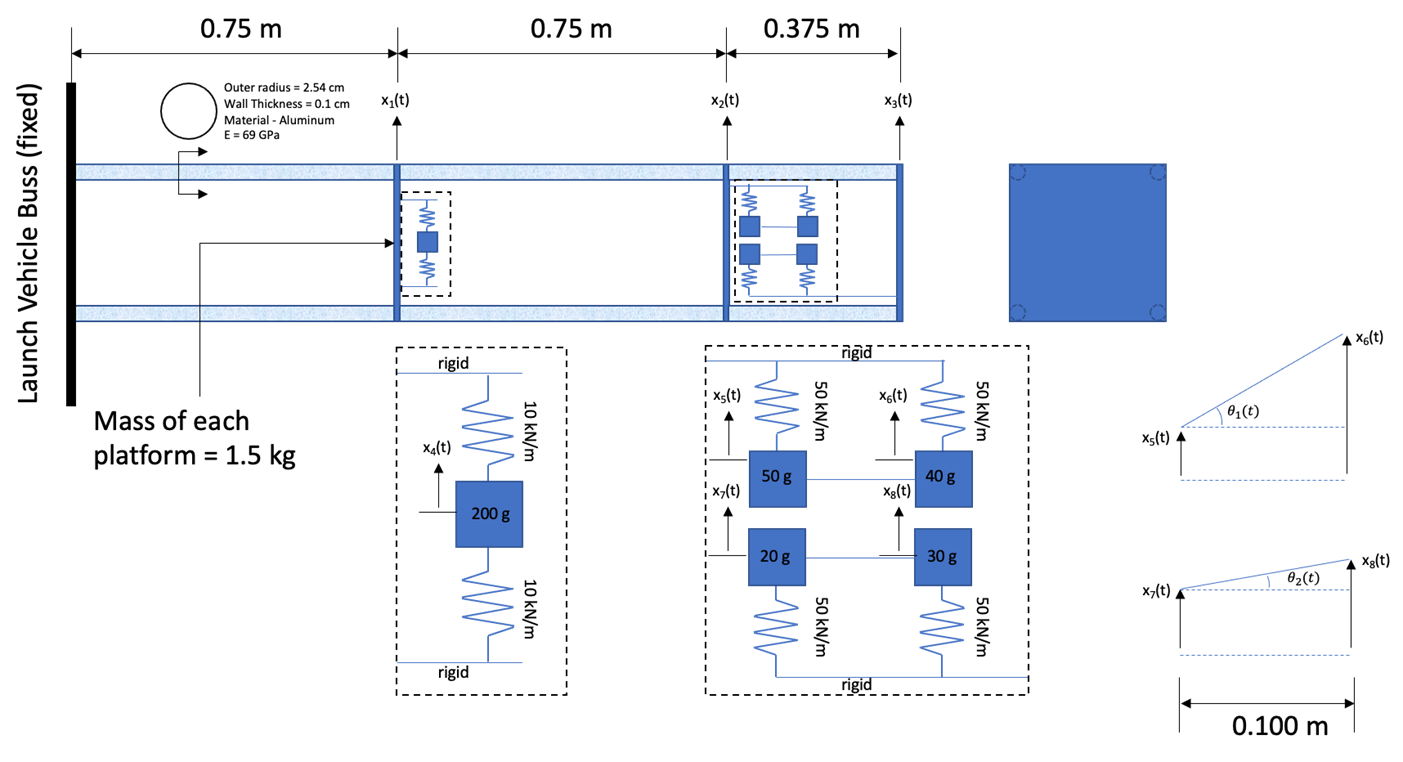
\includegraphics[width=1\textwidth,left]{MCHE 6390/Project 2/Figures/Figure_1.png}
    \captionsetup{justification=raggedright,singlelinecheck=false}
    \caption{Primary System Depiction}
    \label{fig:Main}
\end{figure}

\newpage

Applying our assumptions, we arrive at the following system describing the 3 platforms on the satellite.

\begin{figure}[H]
    \vspace{-10pt}
    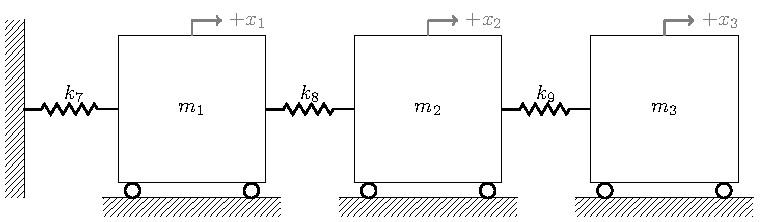
\includegraphics[width=1\textwidth,left]{MCHE 6390/Project 2/Figures/Figure_2.pdf}
    \captionsetup{justification=raggedright,singlelinecheck=false}
    \caption{Platform System}
    \label{fig:Platform}
\end{figure}


\noindent With this lumped parameter model, we can develop equations to describe the system using Lagrange's equations.
\\ \\
\noindent We first determine the kinetic energy in the system,
\begin{flalign*}
    T_{i} &= \frac{1}{2}m_{i}\dot{x}_{i}^{2}.&&
\end{flalign*}
\noindent We now determine the potential energy in the system,
\begin{flalign*}
    U_{1} &= \frac{1}{2}(k_{1}+k_{2})(x_{1}-x_{4})^{2}&& \\
    U_{2} &= \frac{1}{2}k_{3}(x_{5}-x_{2})^{2}&& \\
    U_{3} &= \frac{1}{2}k_{4}(x_{6}-x_{2})^{2}&& \\
    U_{4} &= \frac{1}{2}k_{5}(x_{7}-x_{3})^{2}&& \\
    U_{5} &= \frac{1}{2}k_{6}(x_{8}-x_{3})^{2}&& \\
    U_{6} &= \frac{1}{2}k_{7}x_{1}^{2}&& \\
    U_{7} &= \frac{1}{2}k_{8}(x_{2}-x_{1})^{2}&& \\
    U_{8} &= \frac{1}{2}k_{9}(x_{3}-x_{2})^{2}.&&
\end{flalign*}
\noindent We now assemble the Langrangian as follows,
\begin{flalign*}
    \mathcal{L} &= \displaystyle{\sum_{i=1}^{8}T_{i}}-\displaystyle{\sum_{i=1}^{8}U_{i}}&& \\
    \mathcal{L} &= \displaystyle{\sum_{i=1}^{8}\frac{1}{2}m_{i}\dot{x}_{i}^{2}}-\frac{1}{2}(k_{1}+k_{2})(x_{1}-x_{4})^{2}-\frac{1}{2}k_{3}(x_{5}-x_{2})^{2}-\frac{1}{2}k_{4}(x_{6}-x_{2})^{2}-\frac{1}{2}k_{5}(x_{7}-x_{3})^{2}-\frac{1}{2}k_{6}(x_{8}-x_{3})^{2}-\frac{1}{2}k_{7}x_{1}^{2}&& \\
    &- \frac{1}{2}k_{8}(x_{2}-x_{1})^{2}-\frac{1}{2}k_{9}(x_{3}-x_{2})^{2}.&&
\end{flalign*}
\noindent We now let $q_{i} = x_{i}$ for $i = 1,2,...,8$. We can now write Lagrange's equations as follows,
\begin{flalign*}
    \frac{d}{dt}\left(\frac{\partial\mathcal{L}}{\dot{q}_{i}}\right)-\frac{\partial\mathcal{L}}{{q}_{i}} &= 0&& \\
    \frac{d}{dt}\left(\frac{\partial\mathcal{L}}{\dot{x}_{i}}\right)-\frac{\partial\mathcal{L}}{{x}_{i}} &= 0.&& \\    
\end{flalign*}
\noindent We note that
\begin{flalign*}
    \frac{d}{dt}\left(\frac{\partial\mathcal{L}}{\dot{x}_{i}}\right) &= \frac{d}{dt}\left(\frac{\partial}{\partial \dot{x}_{i}}\displaystyle{\sum_{j=1}^{8}\frac{1}{2}m_{j}\dot{x}_{j}^{2}}\right)= \frac{d}{dt}\left(\displaystyle{\sum_{j=1}^{8}\frac{\partial}{\partial \dot{x}_{i}}\left(\frac{1}{2}m_{j}\dot{x}_{j}^{2}\right)}\right)=\frac{d}{dt}\left(m_{i}\dot{x}_{i}\right)=m_{i}\ddot{x}_{i}.&& \\
\end{flalign*}
\noindent We now calculate $\displaystyle{\frac{\partial \mathcal{L}}{\partial x_{i}}}$,
\begin{flalign*}
    \frac{\partial \mathcal{L}}{\partial x_{1}} &= -(k_{1}+k_{2})(x_{1}-x_{4})-k_{7}x_{1}+k_{8}(x_{2}-x_{1})&& \\
    \frac{\partial \mathcal{L}}{\partial x_{2}} &= k_{3}(x_{5}-x_{2})+k_{4}(x_{6}-x_{2})-k_{8}(x_{2}-x_{1})+k_{9}(x_{3}-x_{2})&& \\
    \frac{\partial \mathcal{L}}{\partial x_{3}} &= k_{5}(x_{7}-x_{3})+k_{6}(x_{8}-x_{3})-k_{9}(x_{3}-x_{2})&& \\
    \frac{\partial \mathcal{L}}{\partial x_{4}} &= (k_{1}+k_2)(x_{1}-x_{4})&& \\
    \frac{\partial \mathcal{L}}{\partial x_{5}} &= -k_{3}(x_{5}-x_{2})&& \\
    \frac{\partial \mathcal{L}}{\partial x_{6}} &= -k_{4}(x_{6}-x_{2})&& \\
    \frac{\partial \mathcal{L}}{\partial x_{7}} &= -k_{5}(x_{7}-x_{3})&& \\
    \frac{\partial \mathcal{L}}{\partial x_{8}} &= -k_{6}(x_{8}-x_{3}).&&
\end{flalign*}
Assembling $\displaystyle{\frac{d}{dt}\left(\frac{\partial\mathcal{L}}{\dot{x}_{i}}\right)-\frac{\partial\mathcal{L}}{{x}_{i}}}$,
\begin{flalign*}
    \frac{d}{dt}\left(\frac{\partial\mathcal{L}}{\dot{x}_{1}}\right)-\frac{\partial\mathcal{L}}{{x}_{1}} &= m_{1}\ddot{x}_{1}+(k_{1}+k_{2})(x_{1}-x_{4})+k_{7}x_{1}-k_{8}(x_{2}-x_{1})=0 && \\
    \frac{d}{dt}\left(\frac{\partial\mathcal{L}}{\dot{x}_{2}}\right)-\frac{\partial\mathcal{L}}{{x}_{2}} &= m_{2}\ddot{x}_{2}-k_{3}(x_{5}-x_{2})-k_{4}(x_{6}-x_{2})+k_{8}(x_{2}-x_{1})-k_{9}(x_{3}-x_{2})=0 && \\
    \frac{d}{dt}\left(\frac{\partial\mathcal{L}}{\dot{x}_{3}}\right)-\frac{\partial\mathcal{L}}{{x}_{3}} &= m_{3}\ddot{x}_{3}-k_{5}(x_{7}-x_{3})-k_{6}(x_{8}-x_{3})+k_{9}(x_{3}-x_{2})=0 && \\
    \frac{d}{dt}\left(\frac{\partial\mathcal{L}}{\dot{x}_{4}}\right)-\frac{\partial\mathcal{L}}{{x}_{4}} &= m_{4}\ddot{x}_{4}-(k_{1}+k_2)(x_{1}-x_{4})=0 && \\
    \frac{d}{dt}\left(\frac{\partial\mathcal{L}}{\dot{x}_{5}}\right)-\frac{\partial\mathcal{L}}{{x}_{5}} &= m_{5}\ddot{x}_{5}+k_{3}(x_{5}-x_{2})=0 && \\
    \frac{d}{dt}\left(\frac{\partial\mathcal{L}}{\dot{x}_{6}}\right)-\frac{\partial\mathcal{L}}{{x}_{6}} &= m_{6}\ddot{x}_{6}+k_{4}(x_{6}-x_{2})=0 && \\
    \frac{d}{dt}\left(\frac{\partial\mathcal{L}}{\dot{x}_{7}}\right)-\frac{\partial\mathcal{L}}{{x}_{7}} &= m_{7}\ddot{x}_{7}+k_{5}(x_{7}-x_{3})=0 && \\
    \frac{d}{dt}\left(\frac{\partial\mathcal{L}}{\dot{x}_{8}}\right)-\frac{\partial\mathcal{L}}{{x}_{8}} &= m_{8}\ddot{x}_{8}+k_{6}(x_{8}-x_{3})=0. && \\
\end{flalign*}
\noindent We now can rewrite our equations of motion by separating terms,
\begin{flalign*}
    &m_{1}\ddot{x}_{1}+(k_{1}+k_{2}+k_{7}+k_{8})x_{1}-k_{8}x_{2}-(k_{1}+k_{2})x_{4}=0 && \\
    &m_{2}\ddot{x}_{2}-k_{8}x_{1}+(k_{4}+k_{5}+k_{8}+k_{9})x_{2}-k_{9}x_{3}-k_{3}x_{5}-k_{4}x_{6}=0 && \\
    &m_{3}\ddot{x}_{3}-k_{9}x_{2}+(k_{5}+k_{6}+k_{9})x_{3}-k_{5}x_{7}-k_{6}x_{8}=0 && \\
    &m_{4}\ddot{x}_{4}-(k_{1}+k_2)x_{1}+(k_{1}+k_2)x_{4}=0 && \\
    &m_{5}\ddot{x}_{5}-k_{3}x_{2}+k_{3}x_{5}=0 && \\
    &m_{6}\ddot{x}_{6}-k_{4}x_{2}+k_{4}x_{6}=0 && \\
    &m_{7}\ddot{x}_{7}-k_{5}x_{3}+k_{5}x_{7}=0 && \\
    &m_{8}\ddot{x}_{8}-k_{6}x_{3}+k_{6}x_{8}=0. && \\
\end{flalign*}
\noindent We can now rewrite our equations of motion in matrix-vector form,
\begin{flalign}
    &
    \begin{bmatrix}
    m_{1} & 0     & 0     & 0     & 0     & 0     & 0     & 0     \\
    0     & m_{2} & 0     & 0     & 0     & 0     & 0     & 0     \\
    0     & 0     & m_{3} & 0     & 0     & 0     & 0     & 0     \\
    0     & 0     & 0     & m_{4} & 0     & 0     & 0     & 0     \\
    0     & 0     & 0     & 0     & m_{5} & 0     & 0     & 0     \\
    0     & 0     & 0     & 0     & 0     & m_{6} & 0     & 0     \\
    0     & 0     & 0     & 0     & 0     & 0     & m_{7} & 0     \\
    0     & 0     & 0     & 0     & 0     & 0     & 0     & m_{8}
    \end{bmatrix}
    \begin{bmatrix}
    \ddot{x}_{1} \\
    \ddot{x}_{2} \\
    \ddot{x}_{3} \\
    \ddot{x}_{4} \\
    \ddot{x}_{5} \\
    \ddot{x}_{6} \\
    \ddot{x}_{7} \\
    \ddot{x}_{8}
    \end{bmatrix}
    +
    && \nonumber \\
    &
    \begin{bmatrix}
    k_{1}+k_{2}+k_{7}+k_{8} & -k_{8}                               & 0                 & -k_{1}-k_{2} & 0      & 0      & 0      & 0      \\
    -k_{8}                  & k_{4}+k_{5}+k_{8}+k_{9}              & -k_{9}            & 0            & -k_{3} & -k_{4} & 0      & 0      \\
    0                       & -k_{9}                               & k_{5}+k_{6}+k_{9} & 0            & 0      & 0      & -k_{5} & -k_{6} \\
    -k_{1}-k_{2}            & 0                                    & 0                 & k_{1}+k_{2}  & 0      & 0      & 0      & 0      \\
    0                       & -k_{3}                               & 0                 & 0            & k_{3}  & 0      & 0      & 0      \\
    0                       & -k_{4}                               & 0                 & 0            & 0      & k_{4}  & 0      & 0      \\
    0                       & 0                                    & -k_{5}            & 0            & 0      & 0      & k_{5}  & 0      \\
    0                       & 0                                    & -k_{6}            & 0            & 0      & 0      & 0      & k_{6}
    \end{bmatrix}
    \begin{bmatrix}
    x_{1} \\
    x_{2} \\
    x_{3} \\
    x_{4} \\
    x_{5} \\
    x_{6} \\
    x_{7} \\
    x_{8}
    \end{bmatrix}
    =
    \begin{bmatrix}
    0 \\
    0 \\
    0 \\
    0 \\
    0 \\
    0 \\
    0 \\
    0
    \end{bmatrix}.
    && \label{eq:EOM}
\end{flalign}

With this, we can now calculate our mass and stiffness matrices.

Given is the equation for equivalent stiffness of a fixed-fixed beam,
\begin{flalign}
    k_{eq} &= \alpha \frac{EI}{l^{3}},&& \label{eq:k_eq_ff}
\end{flalign}
where $\alpha = 12$.

Substituting in the equation for moment of inertia of an annular section,
\begin{flalign}
    I_{\text{ann}} &= \frac{\pi}{4}\left(r_{o}^{4}-r_{i}^{4}\right), \nonumber
\end{flalign}
into \fref{eq:k_eq_ff}, we arrive at
\begin{flalign}
    k_{eq_{\text{ann}}} &= \frac{3\pi E(r_{o}^{4}-r_{i}^{4})}{l^{3}}.
\end{flalign}
And finally applying the fact that there are four beams of equivalent stiffness attached to each platform, we come up with the final expression,
\begin{flalign}
    k_{eq_{\text{ann,f}}} &= \frac{12\pi E(r_{o}^{4}-r_{i}^{4})}{l^{3}}.
\end{flalign}
Using the code given in the appendix and the dimensions provided to us, we can come up with the following equivalent stiffnesses
\begin{flalign*}
    \begin{bmatrix}
    k_{7} \\
    k_{8} \\
    k_{9}     
    \end{bmatrix}
    &=
    \begin{bmatrix}
    380916 \\
    380916 \\
    304733   
    \end{bmatrix}\text{N/m}.
\end{flalign*}
Substituting these values into our matrix, along with the given stiffnesses, we can come up with the final stiffness matrix,
\begin{flalign*}
    K = 
    \begin{bmatrix}
    781833  & -380916  & 0        & -20000 & 0      & 0      & 0      & 0      \\
    -380916 & 3528247  & -3047330 & 0      & -50000 & -50000 & 0      & 0      \\
    0       & -3047330 & 3147330  & 0      & 0      & 0      & -50000 & -50000 \\
    -20000  & 0        & 0        & 20000  & 0      & 0      & 0      & 0      \\
    0       & -50000   & 0        & 0      & 50000  & 0      & 0      & 0      \\
    0       & -50000   & 0        & 0      & 0      & 50000  & 0      & 0      \\
    0       & 0        & -50000   & 0      & 0      & 0      & 50000  & 0      \\
    0       & 0        & -50000   & 0      & 0      & 0      & 0      & 50000
    \end{bmatrix}
    \text{N/m}.
\end{flalign*}
Substituting given masses, we can come up with the final mass matrix,
\begin{flalign*}
    M = 
    \begin{bmatrix}
    1.5   & 0     & 0     & 0     & 0     & 0     & 0     & 0     \\
    0     & 1.5   & 0     & 0     & 0     & 0     & 0     & 0     \\
    0     & 0     & 1.5   & 0     & 0     & 0     & 0     & 0     \\
    0     & 0     & 0     & 0.2   & 0     & 0     & 0     & 0     \\
    0     & 0     & 0     & 0     & 0.05  & 0     & 0     & 0     \\
    0     & 0     & 0     & 0     & 0     & 0.04  & 0     & 0     \\
    0     & 0     & 0     & 0     & 0     & 0     & 0.02  & 0     \\
    0     & 0     & 0     & 0     & 0     & 0     & 0     & 0.03
    \end{bmatrix}
    \text{kg}.
\end{flalign*}
\newpage
\section*{Natural Frequency and Modal Response Classification}

\noindent Using the code available in the appendix, we now determine our natural frequencies and mode shapes

\begin{flalign*}
    \begin{bmatrix}
    f_{n_{1}} \\
    f_{n_{2}} \\
    f_{n_{3}} \\
    f_{n_{4}} \\
    f_{n_{5}} \\
    f_{n_{6}} \\
    f_{n_{7}} \\
    f_{n_{8}}
    \end{bmatrix}
    &=
    \begin{bmatrix}
    35.94 \\
    50.76 \\
    120.74 \\
    160.02 \\
    178.51 \\
    206.24 \\
    251.59 \\
    330.56
    \end{bmatrix}Hz.
    && \\
    \begin{bmatrix}
    U_{1} \\
    U_{2} \\
    U_{3} \\
    U_{4} \\
    U_{5} \\
    U_{6} \\
    U_{7} \\
    U_{8}
    \end{bmatrix}&^{T}
    =
    \begin{bmatrix}
    0.2865 & 0.2010  & 0.7623  & -0.0250 & 0.0110  & 0.0220  & -0.0148 & -0.0393 \\
    0.4999 & 0.1478  & -0.1545 & 0.0481  & -0.0319 & -0.1004 & 0.1153  & 0.5869  \\
    0.5132 & 0.1558  & -0.2198 & 0.1032  & -0.1016 & -0.0432 & -0.0033 & -0.5549 \\
    0.5848 & -2.1523 & -0.1603 & 0.0027  & 0       & -0.0014 & 0       & 0       \\
    0.5267 & 0.1644  & -0.3640 & -4.4146 & 0.1235  & 0.1477  & -0.0769 & -0.1771 \\
    0.5211 & 0.1607  & -0.2864 & 0.2513  & 4.9398  & 0.2922  & -0.1154 & -0.2394 \\
    0.5239 & 0.1623  & -0.2855 & 0.1732  & -0.2045 & -0.1316 & -6.9960 & 0.7648  \\
    0.5294 & 0.1658  & -0.3357 & 0.2622  & -0.4145 & 5.7053  & 0.0066  & 0.3494.
    \end{bmatrix} &&
\end{flalign*}
\noindent In order to classify the modes, we divided the system into 3 parts. The first part consists of the 3 platform system supporting the other instruments. The second part is the first instrument and the third part are the two bars connecting the second set of instruments.
\\
\\
\noindent When classifying the mode shapes of the platform, we determined first what the "curvature" near the end was. This curvature was determined by looking at the sign of the final two degrees of freedom in the platform model (i.e. $x_{2}$ and $x_{3}$). Positive curvature was assigned to those modes who had increasing displacements near the end, whereas negative curvature was assigned to those modes who had decreasing displacements near the end. We then determined how many sign crossings there were and used that to determine the number of nodes we have. Note that, as expected, the number of nodes increases with the mode number as these are higher energy modes.
\\
\\
\noindent The final thing we would like to note is that the fourth degree of freedom is quite an interesting case. This is a result of the fact that we are modeling the bars attaching $m_{5}$,$m_{6}$,$m_{7}$, and $m_{8}$ as perfectly rigid, and therefore these masses have no way to influence the fourth degree of freedom. 

\begin{table}[H]
    \centering
    \begin{tabular}{|M{1.75cm}|M{1.75cm}||M{1.75cm}|M{1.75cm}|M{2cm}|M{2cm}|M{2cm}|}
        \hline
        Mode Number & Natural Frequency & Platform Boundary Curvature & Number of Platform Nodes & Instrument 1 Position & $\theta_{1}$ & $\theta_{2}$\\
        \hline
        \hline
        1 & 35.94 & + & 0 & + & - & + \\
        \hline
        2 & 50.76 & + & 0 & - & - & + \\
        \hline
        3 & 120.74 & - & 1 & - & + & - \\
        \hline
        4 & 160.02 & + & 1 & + & + & + \\
        \hline
        5 & 178.51 & - & 1 & Node  & + & - \\
        \hline
        6 & 206.24 & + & 1 & $\sim$Node & + & + \\
        \hline
        7 & 251.59 & - & 2 & Node & - & +\\
        \hline
        8 & 330.56 & - & 2 & Node & - & -\\
        \hline
    \end{tabular}
    \caption{Modal Classification Chart}
    \label{tab:Modal_Classification_Chart}
\end{table}


\section*{Damping Design and Relevant Graphic with Cost}
\noindent In order to optimize for cost, we set up a set of nonlinear equations using \fmin. We first determine our constraints,
\begin{flalign*}
    \left(\theta_{2}-\theta_{2}\right)_{RMS} &= 0.2 = \frac{1}{N}\displaystyle{\sum_{i}^{N}\left(\text{\atand}(x_{6_{i}}-x_{5_{i}},0.1)-\text{\atand}(x_{8_{i}}-x_{7_{i}},0.1)\right)^{2}}&& \\
    \max{x_{4_{i}}} &= 0.002.&&
\end{flalign*}
\noindent Since \fmin \,requires for the constraint functions to equal 0, so we subtract off the constraints and obtain
\begin{flalign*}
    0 &= -0.2+\frac{1}{N}\displaystyle{\sum_{i}^{N}\left(\text{\atand}(x_{6_{i}}-x_{5_{i}},0.1)-\text{\atand}(x_{8_{i}}-x_{7_{i}},0.1)\right)^{2}}&& \\
    0 &= -0.002+\max{x_{4_{i}}}.&&
\end{flalign*}
\noindent We now define our objective function,
\begin{flalign*}
    f_{obj} &= \$100,000\sum_{i=1}^{8}\left(\zeta_{i}-0.001\right)^{2}.
\end{flalign*}
\noindent Using the code in the appendix, we obtain the following damping coefficients,
\begin{flalign*}
    \begin{bmatrix}
    \zeta_{1} \\
    \zeta_{2} \\
    \zeta_{3} \\
    \zeta_{4} \\
    \zeta_{5} \\
    \zeta_{6} \\
    \zeta_{7} \\
    \zeta_{8}
    \end{bmatrix}
    &=
    \begin{bmatrix}
    0.3188 \\
    0.1214 \\
    0.0042 \\
    0.1409 \\
    0.2088 \\
    0.2544 \\
    0.2289 \\
    0.0087
    \end{bmatrix}.
\end{flalign*}
\noindent Per our cost function, this treatment will cost \$29,446.37. It will additionally have $\theta_{RMS}=0.1986\deg$ and $\max{x_{4_{i}}}=1.24$mm.
\\
\\
\noindent We now compare the responses in $x_{4}$ and $\theta_1-\theta_{2}$ with and without damping,
\begin{figure}[H]
    \vspace{-10pt}
    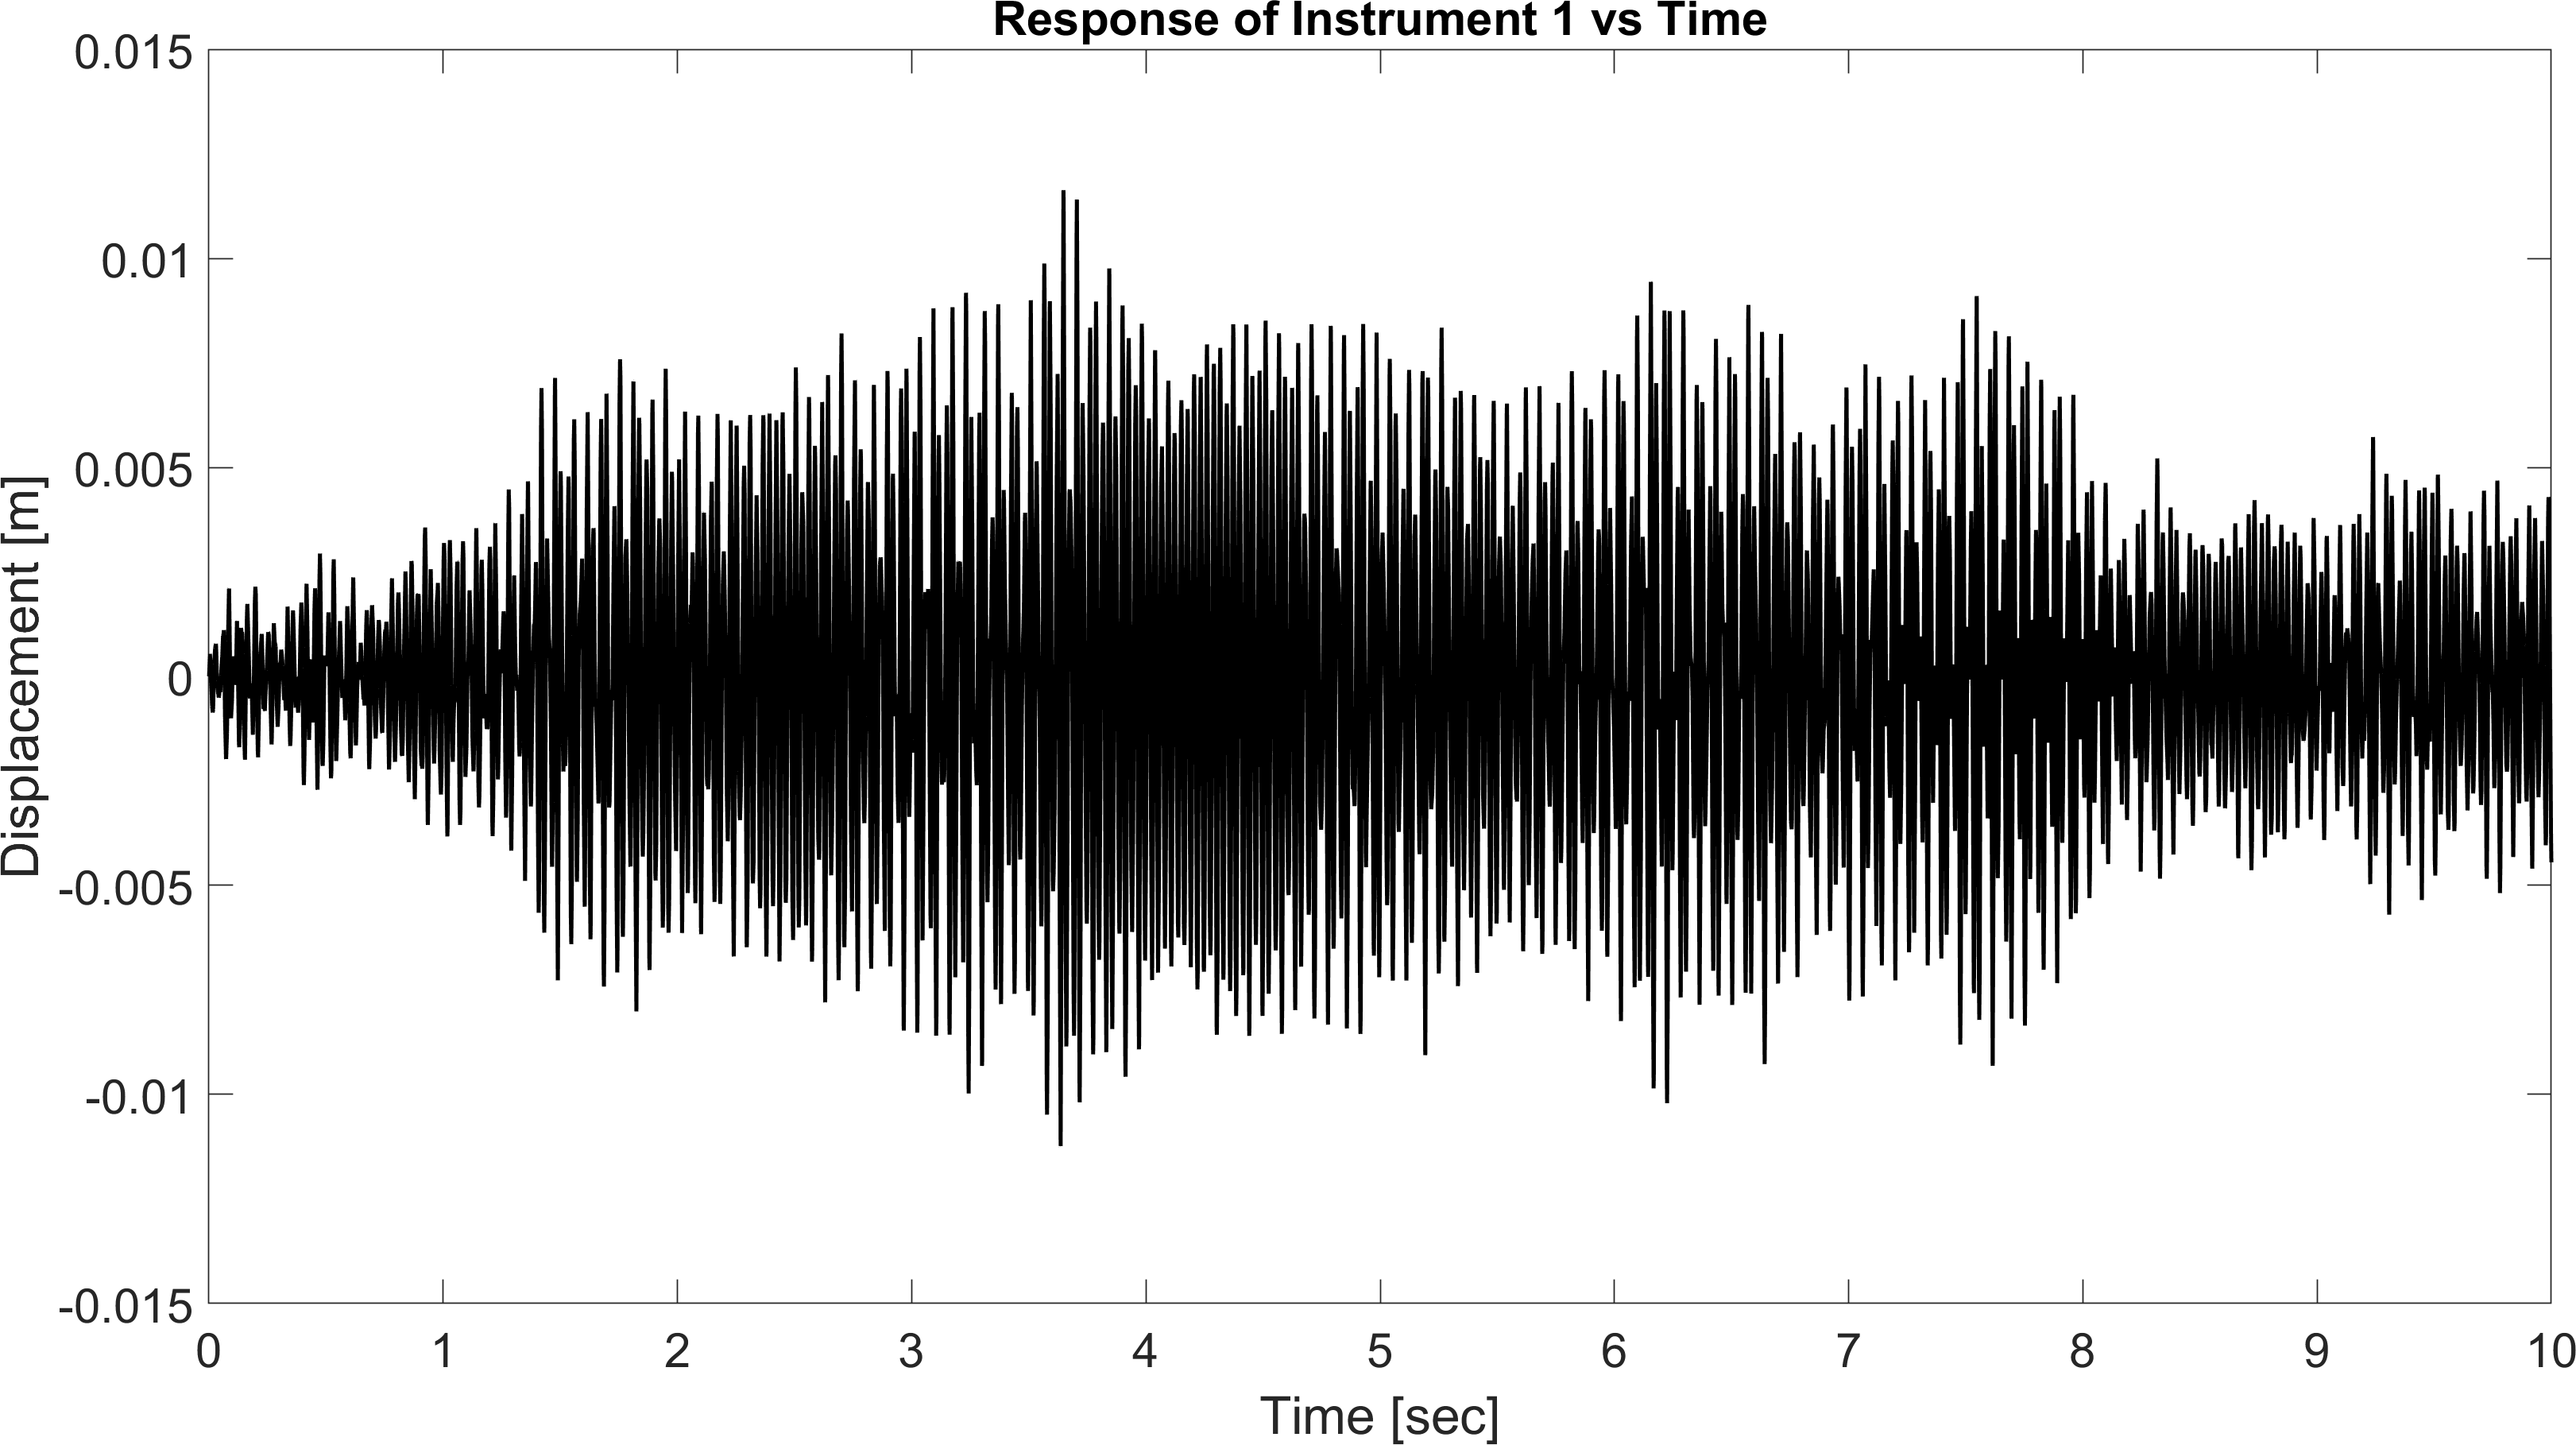
\includegraphics[width=1\textwidth,left]{MCHE 6390/Project 2/Figures/Figure_3.png}
    \captionsetup{justification=raggedright,singlelinecheck=false}
    \caption{$x_{4}$ without damping}
    \label{fig:x4nodamp}
\end{figure}
\begin{figure}[H]
    \vspace{-10pt}
    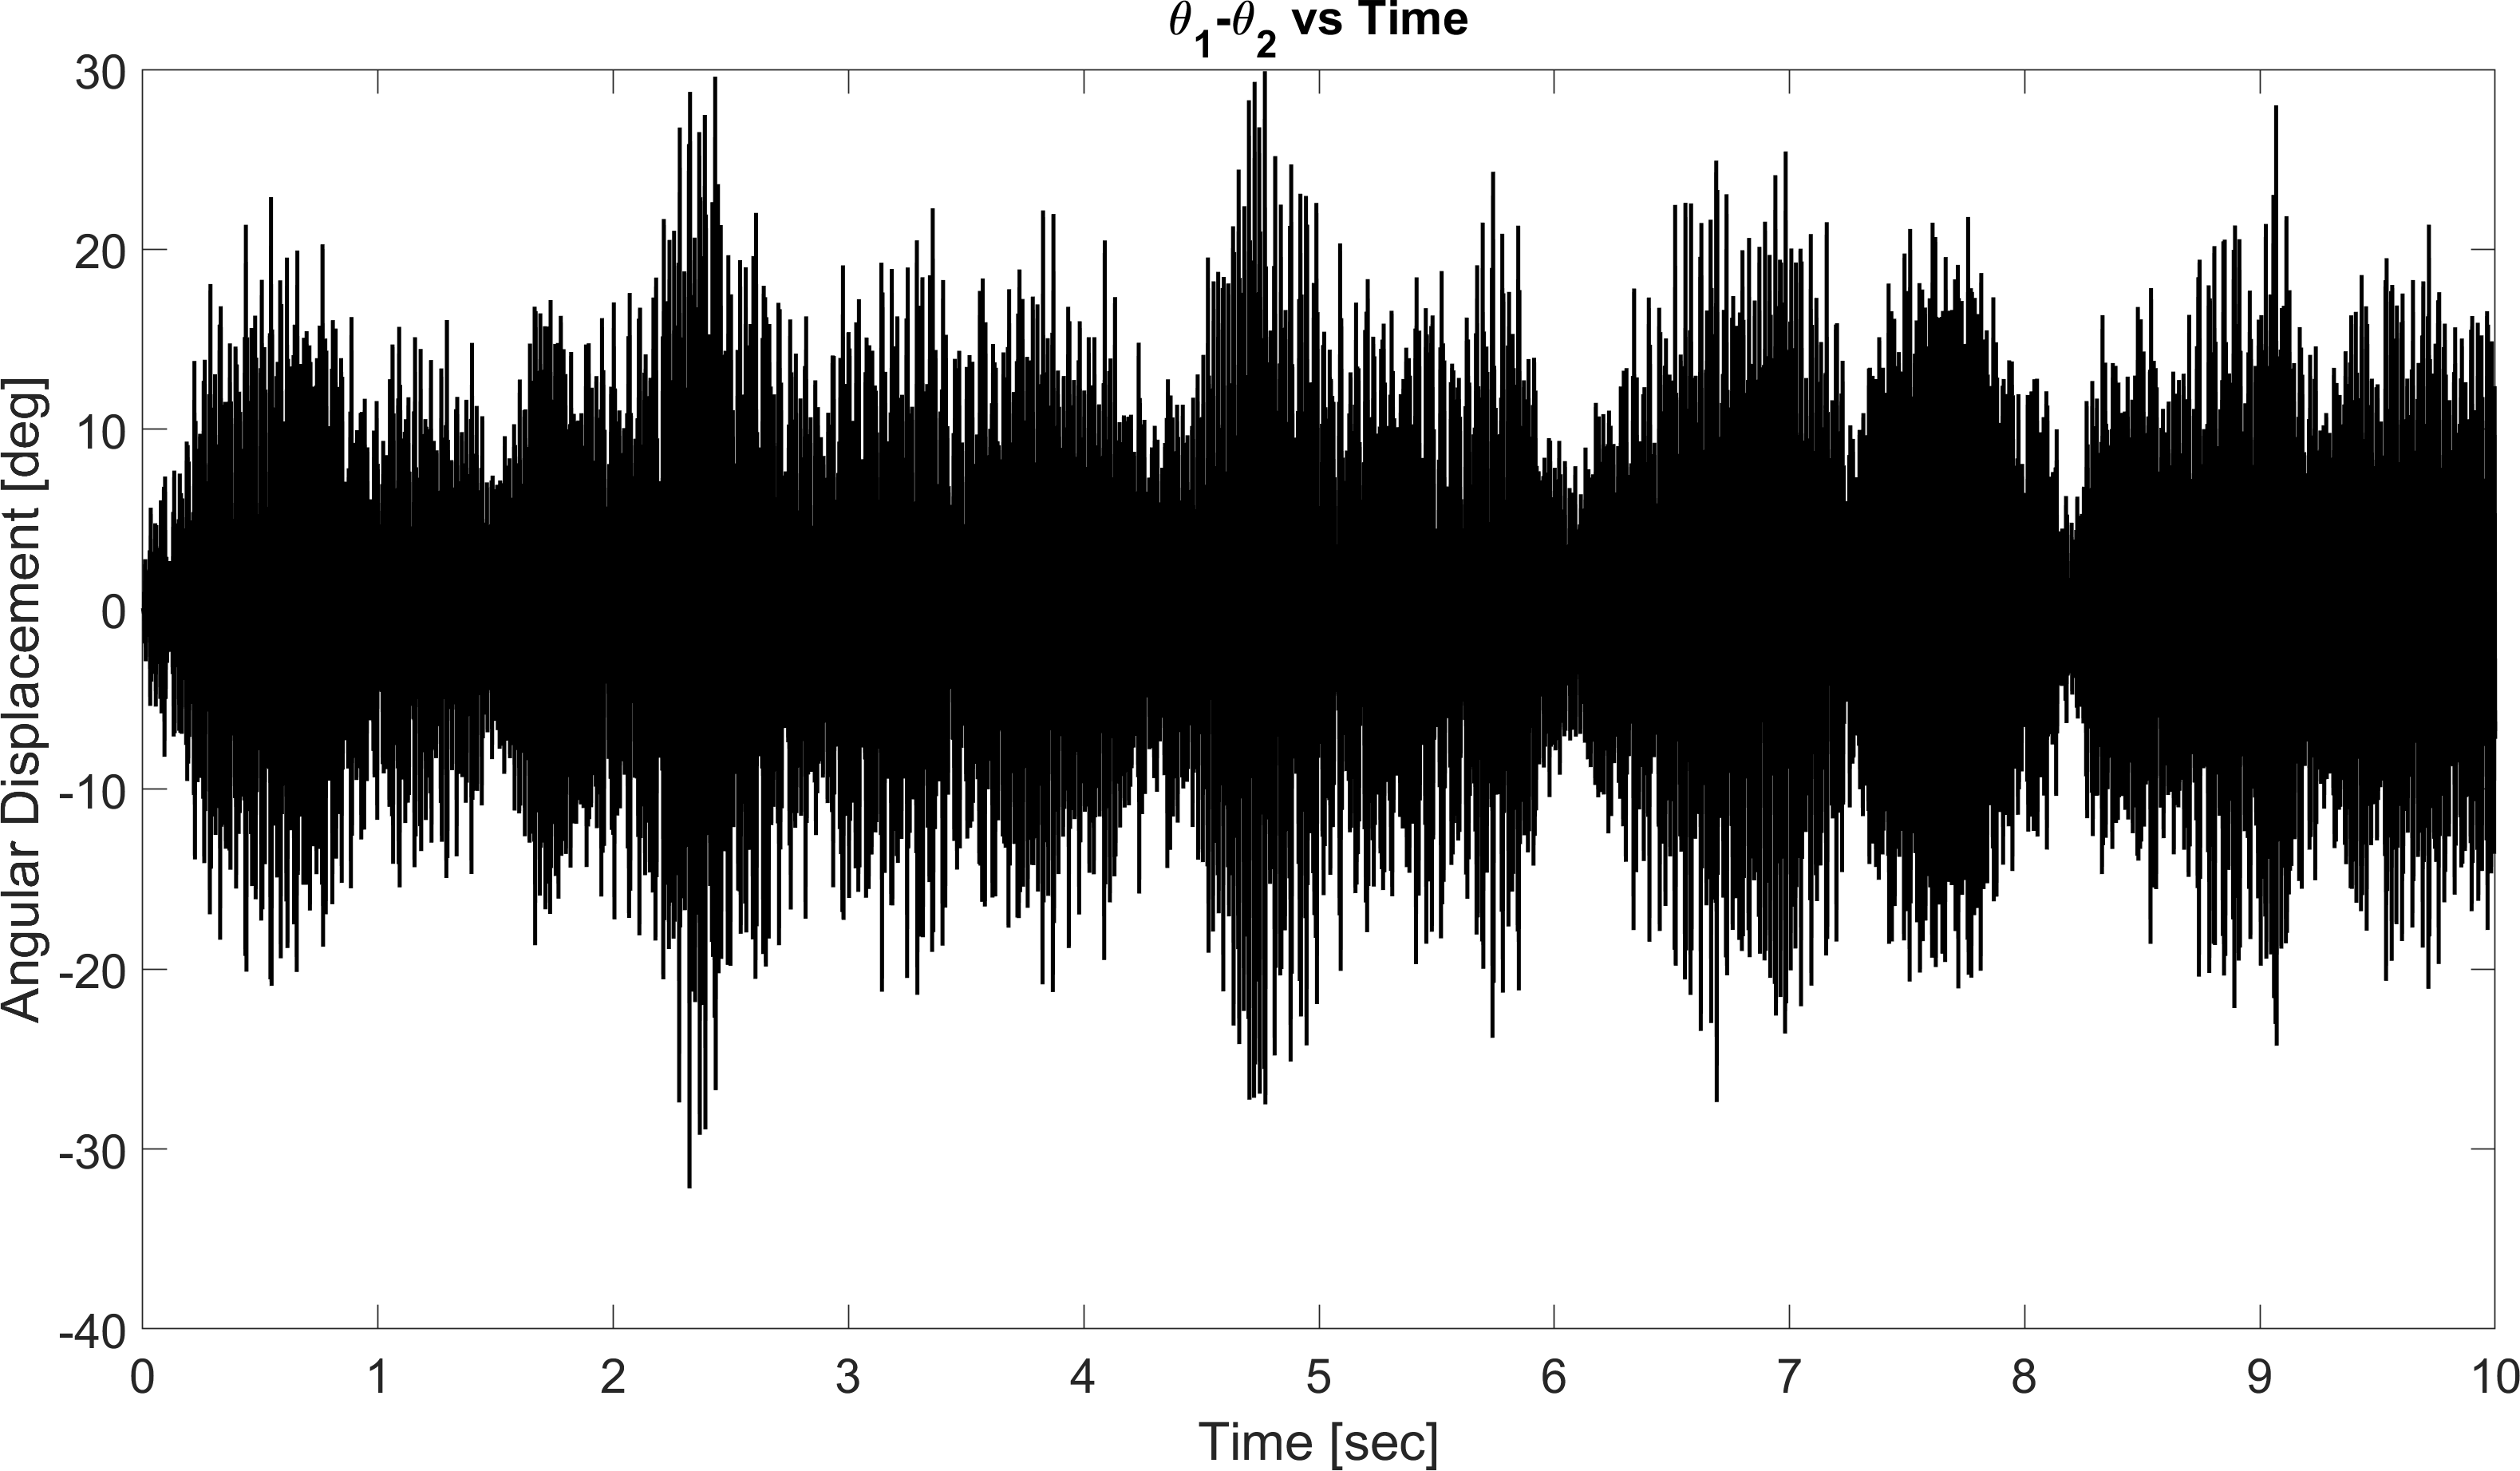
\includegraphics[width=1\textwidth,left]{MCHE 6390/Project 2/Figures/Figure_4.png}
    \captionsetup{justification=raggedright,singlelinecheck=false}
    \caption{$\theta_{1}-\theta_{2}$ without damping}
    \label{fig:t1t2nodamp}
\end{figure}
\begin{figure}[H]
    \vspace{-10pt}
    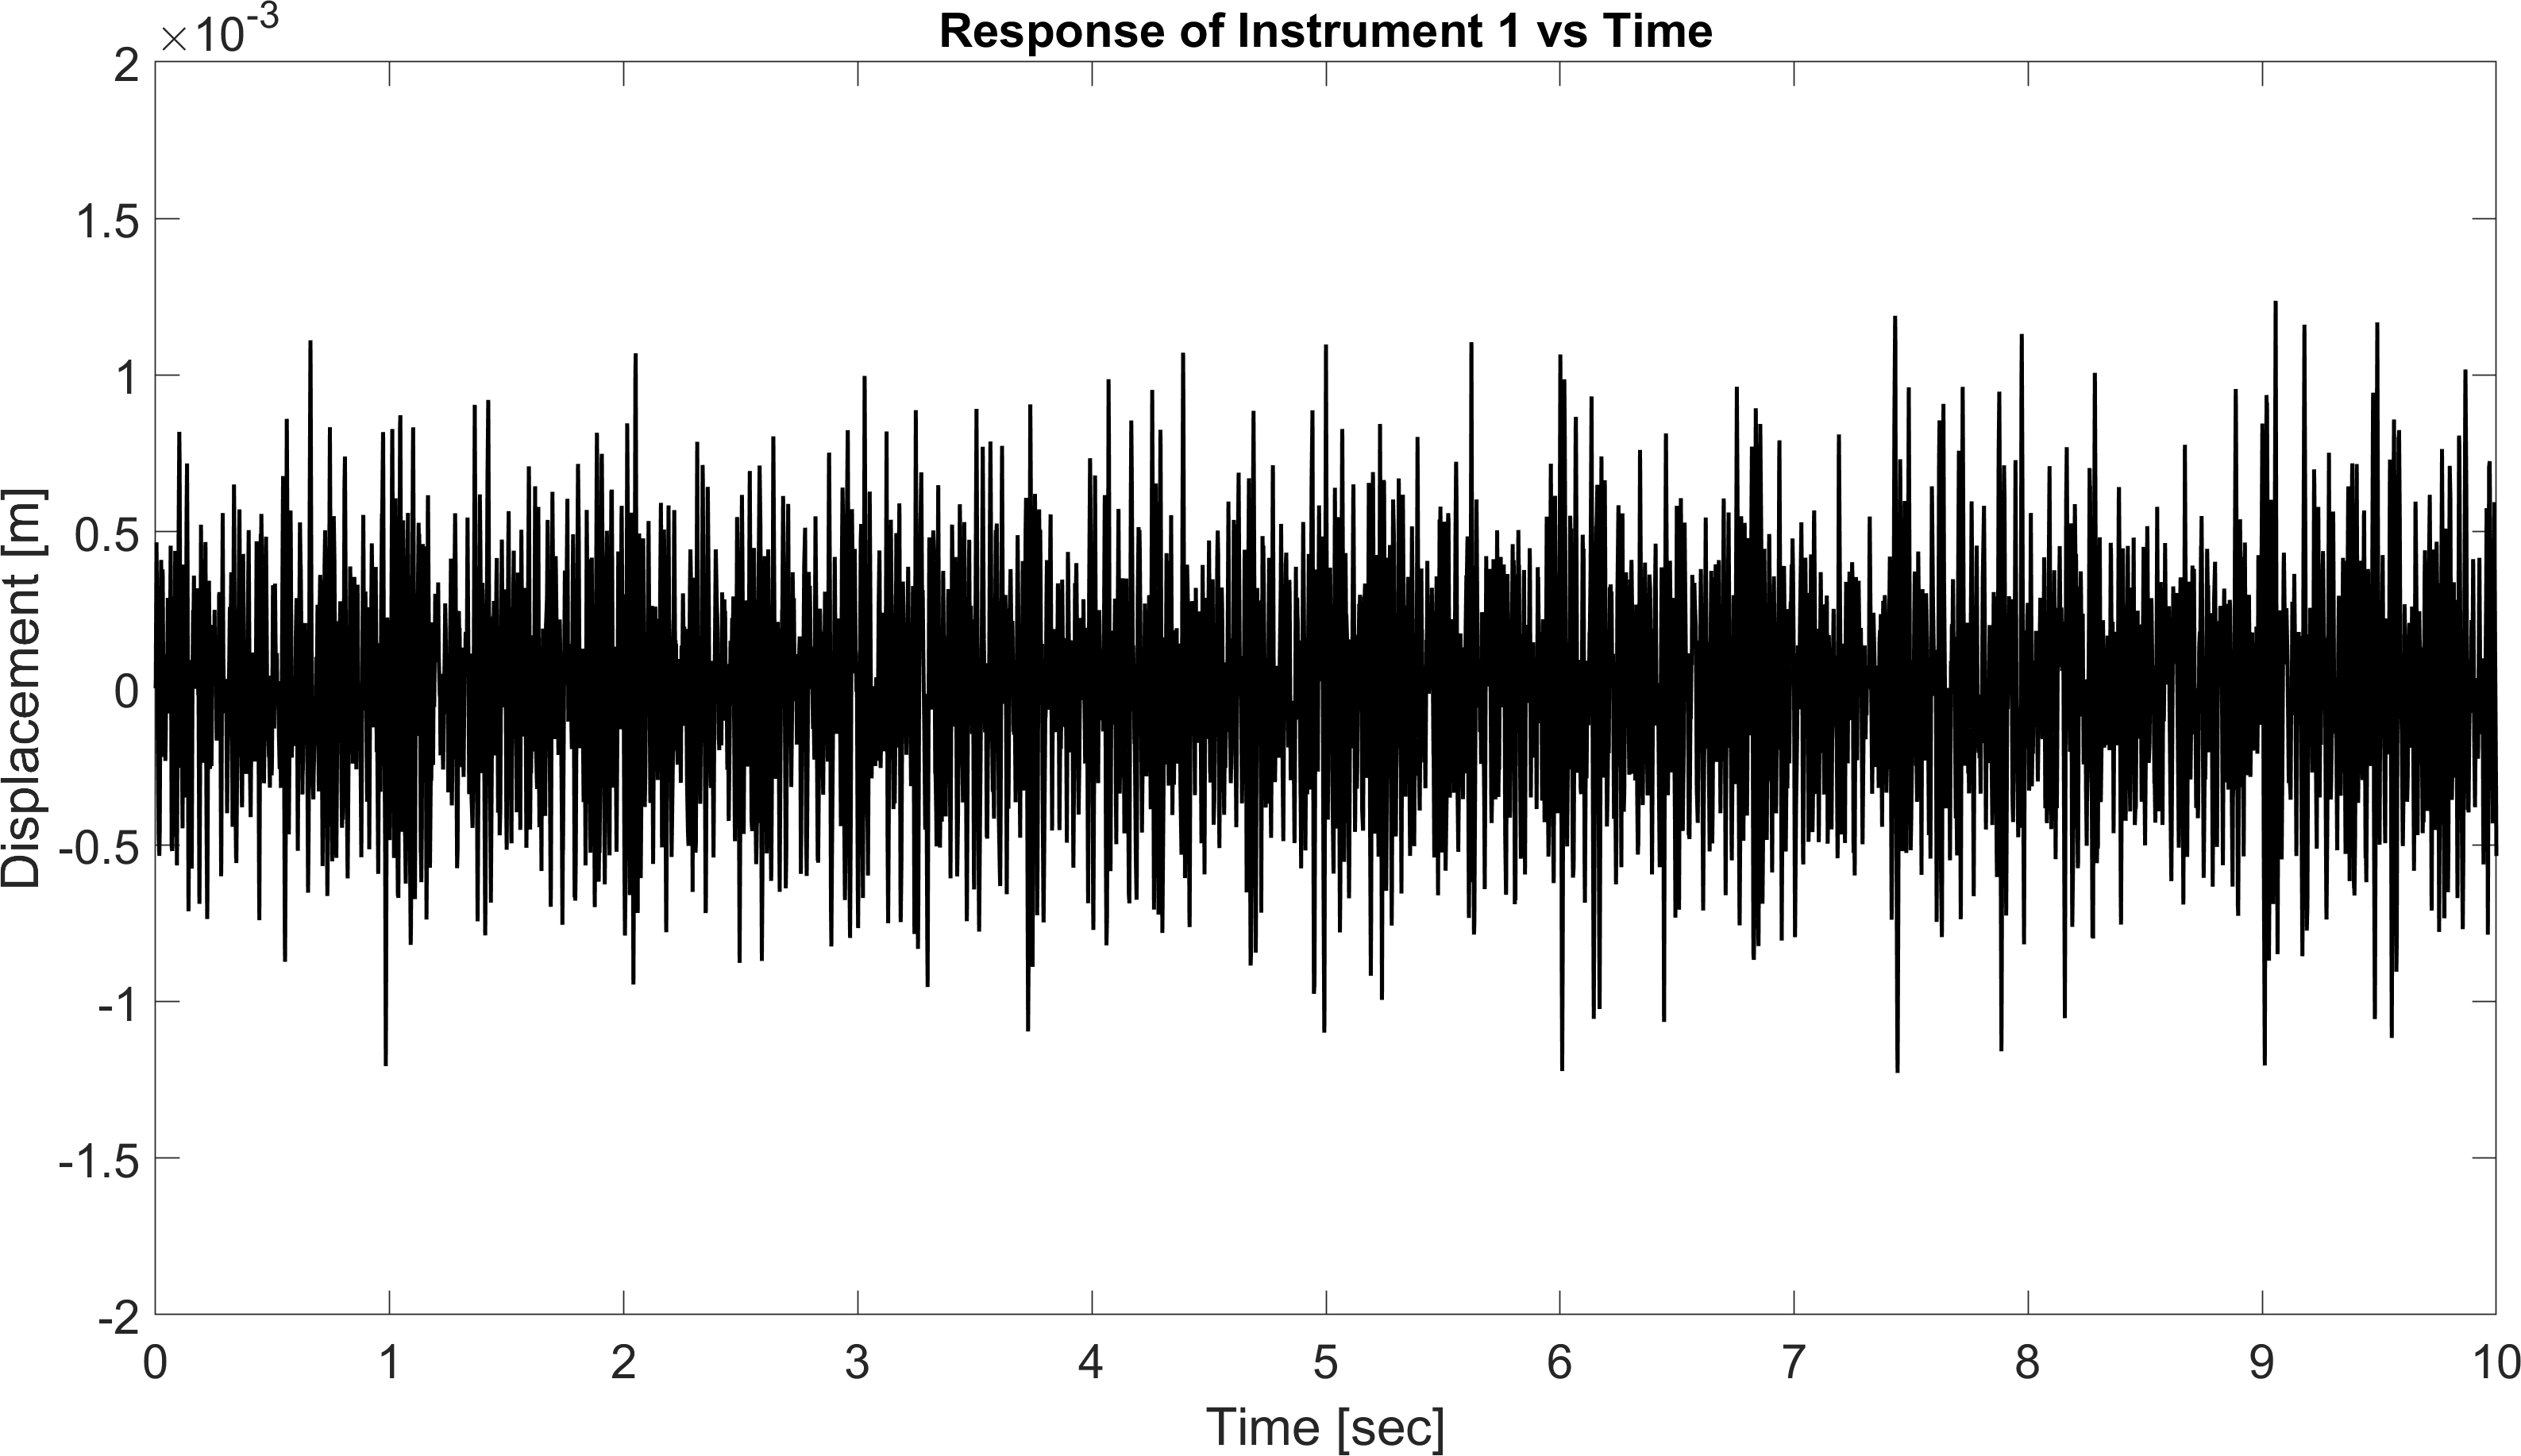
\includegraphics[width=1\textwidth,left]{MCHE 6390/Project 2/Figures/Figure_5.png}
    \captionsetup{justification=raggedright,singlelinecheck=false}
    \caption{$x_{4}$ with the damping treatment}
    \label{fig:x4damp}
\end{figure}
\begin{figure}[H]
    \vspace{-10pt}
    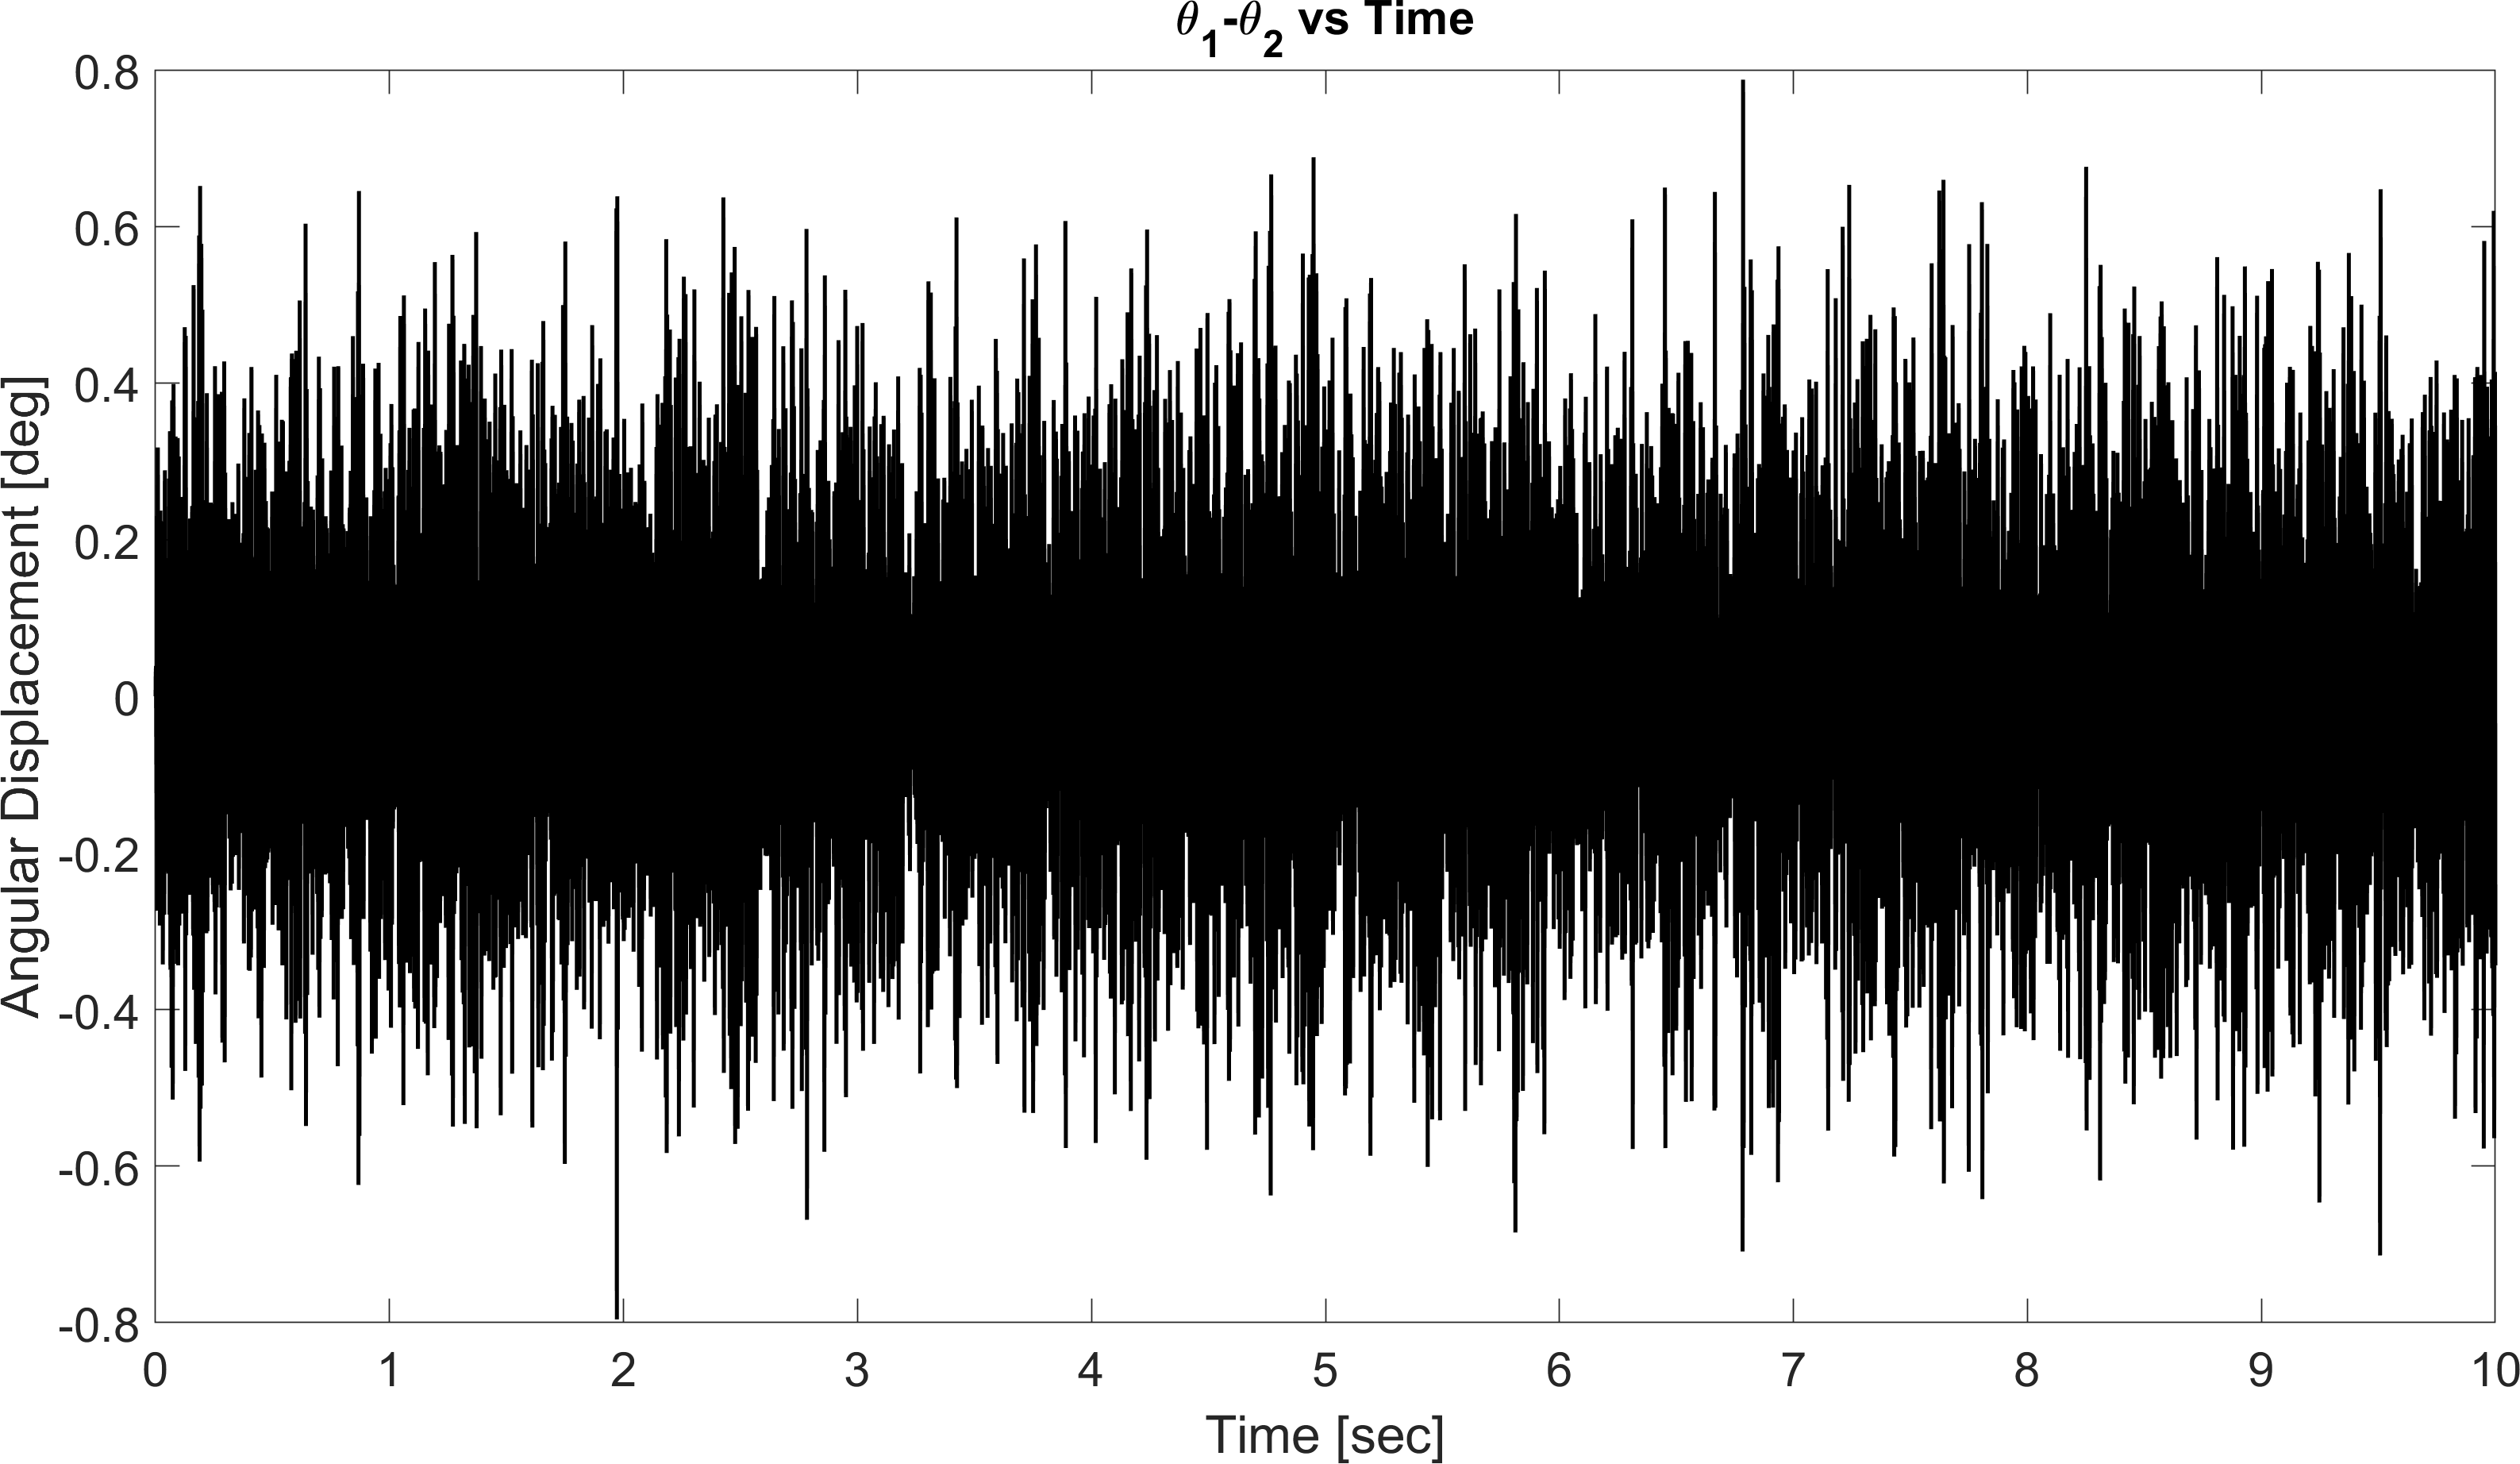
\includegraphics[width=1\textwidth,left]{MCHE 6390/Project 2/Figures/Figure_6.png}
    \captionsetup{justification=raggedright,singlelinecheck=false}
    \caption{$\theta_{1}-\theta_{2}$ with the damping treatment}
    \label{fig:t1t2damp}
\end{figure}

\noindent It will prudent for us to confirm these results. The primary step we would like to verify is the convolution step. In order to do this, we will take a basic model that we know the response to and compare the results to our algorithm. With this in mind, take
\begin{flalign*}
    &
    \begin{bmatrix}
    1 & 0 \\
    0 & 1 \\
    \end{bmatrix}
    \begin{bmatrix}
    \ddot{r}_{1} \\
    \ddot{r}_{2} \\
    \end{bmatrix}
    +
    \begin{bmatrix}
    4 & 0 \\
    0 & 9 \\
    \end{bmatrix}
    \begin{bmatrix}
    r_{1} \\
    r_{1} \\
    \end{bmatrix}
    =
    \begin{bmatrix}
    0 \\
    0 \\
    \end{bmatrix}.
\end{flalign*}
\noindent Additionally, take
\begin{flalign*}
    U &=
    \begin{bmatrix}
    1 & 2 \\
    3 & -1 \\
    \end{bmatrix}&& \\
    \begin{bmatrix}
    \zeta_{1} \\
    \zeta_{2} \\
    \end{bmatrix}
    &=
    \begin{bmatrix}
    0 \\
    0 \\
    \end{bmatrix} && \\
    B_{f} &= 
    \begin{bmatrix}
    0 \\
    1 \\
    \end{bmatrix}&& \\
    \begin{bmatrix}
    \ddot{r}_{1}(0) \\
    \ddot{r}_{2}(0) \\
    \end{bmatrix}
    &=
    \begin{bmatrix}
    0 \\
    0 \\
    \end{bmatrix} && \\
    \begin{bmatrix}
    r_{1}(0) \\
    r_{2}(0) \\
    \end{bmatrix}
    &=
    \begin{bmatrix}
    0 \\
    0 \\
    \end{bmatrix} && \\
    f(t) &= 5u(t) &&
\end{flalign*}
\noindent Analytically, we know that our solution is
\begin{flalign*}
    \begin{bmatrix}
    x_{1}(t) \\
    x_{2}(t) \\
    \end{bmatrix}
    &=
    \begin{bmatrix}
    2.5-2.5\cos(2t)-\frac{5}{3}+\frac{5}{3}\cos(3t) \\
    5-5\cos(2t)+\frac{5}{9}-\frac{5}{9}\cos(3t)
    \end{bmatrix}.
\end{flalign*}

\noindent Comparing the solutions and normalizing by the magnitude of the analytical response, we arrive at the following.
\begin{figure}[H]
    \vspace{-10pt}
    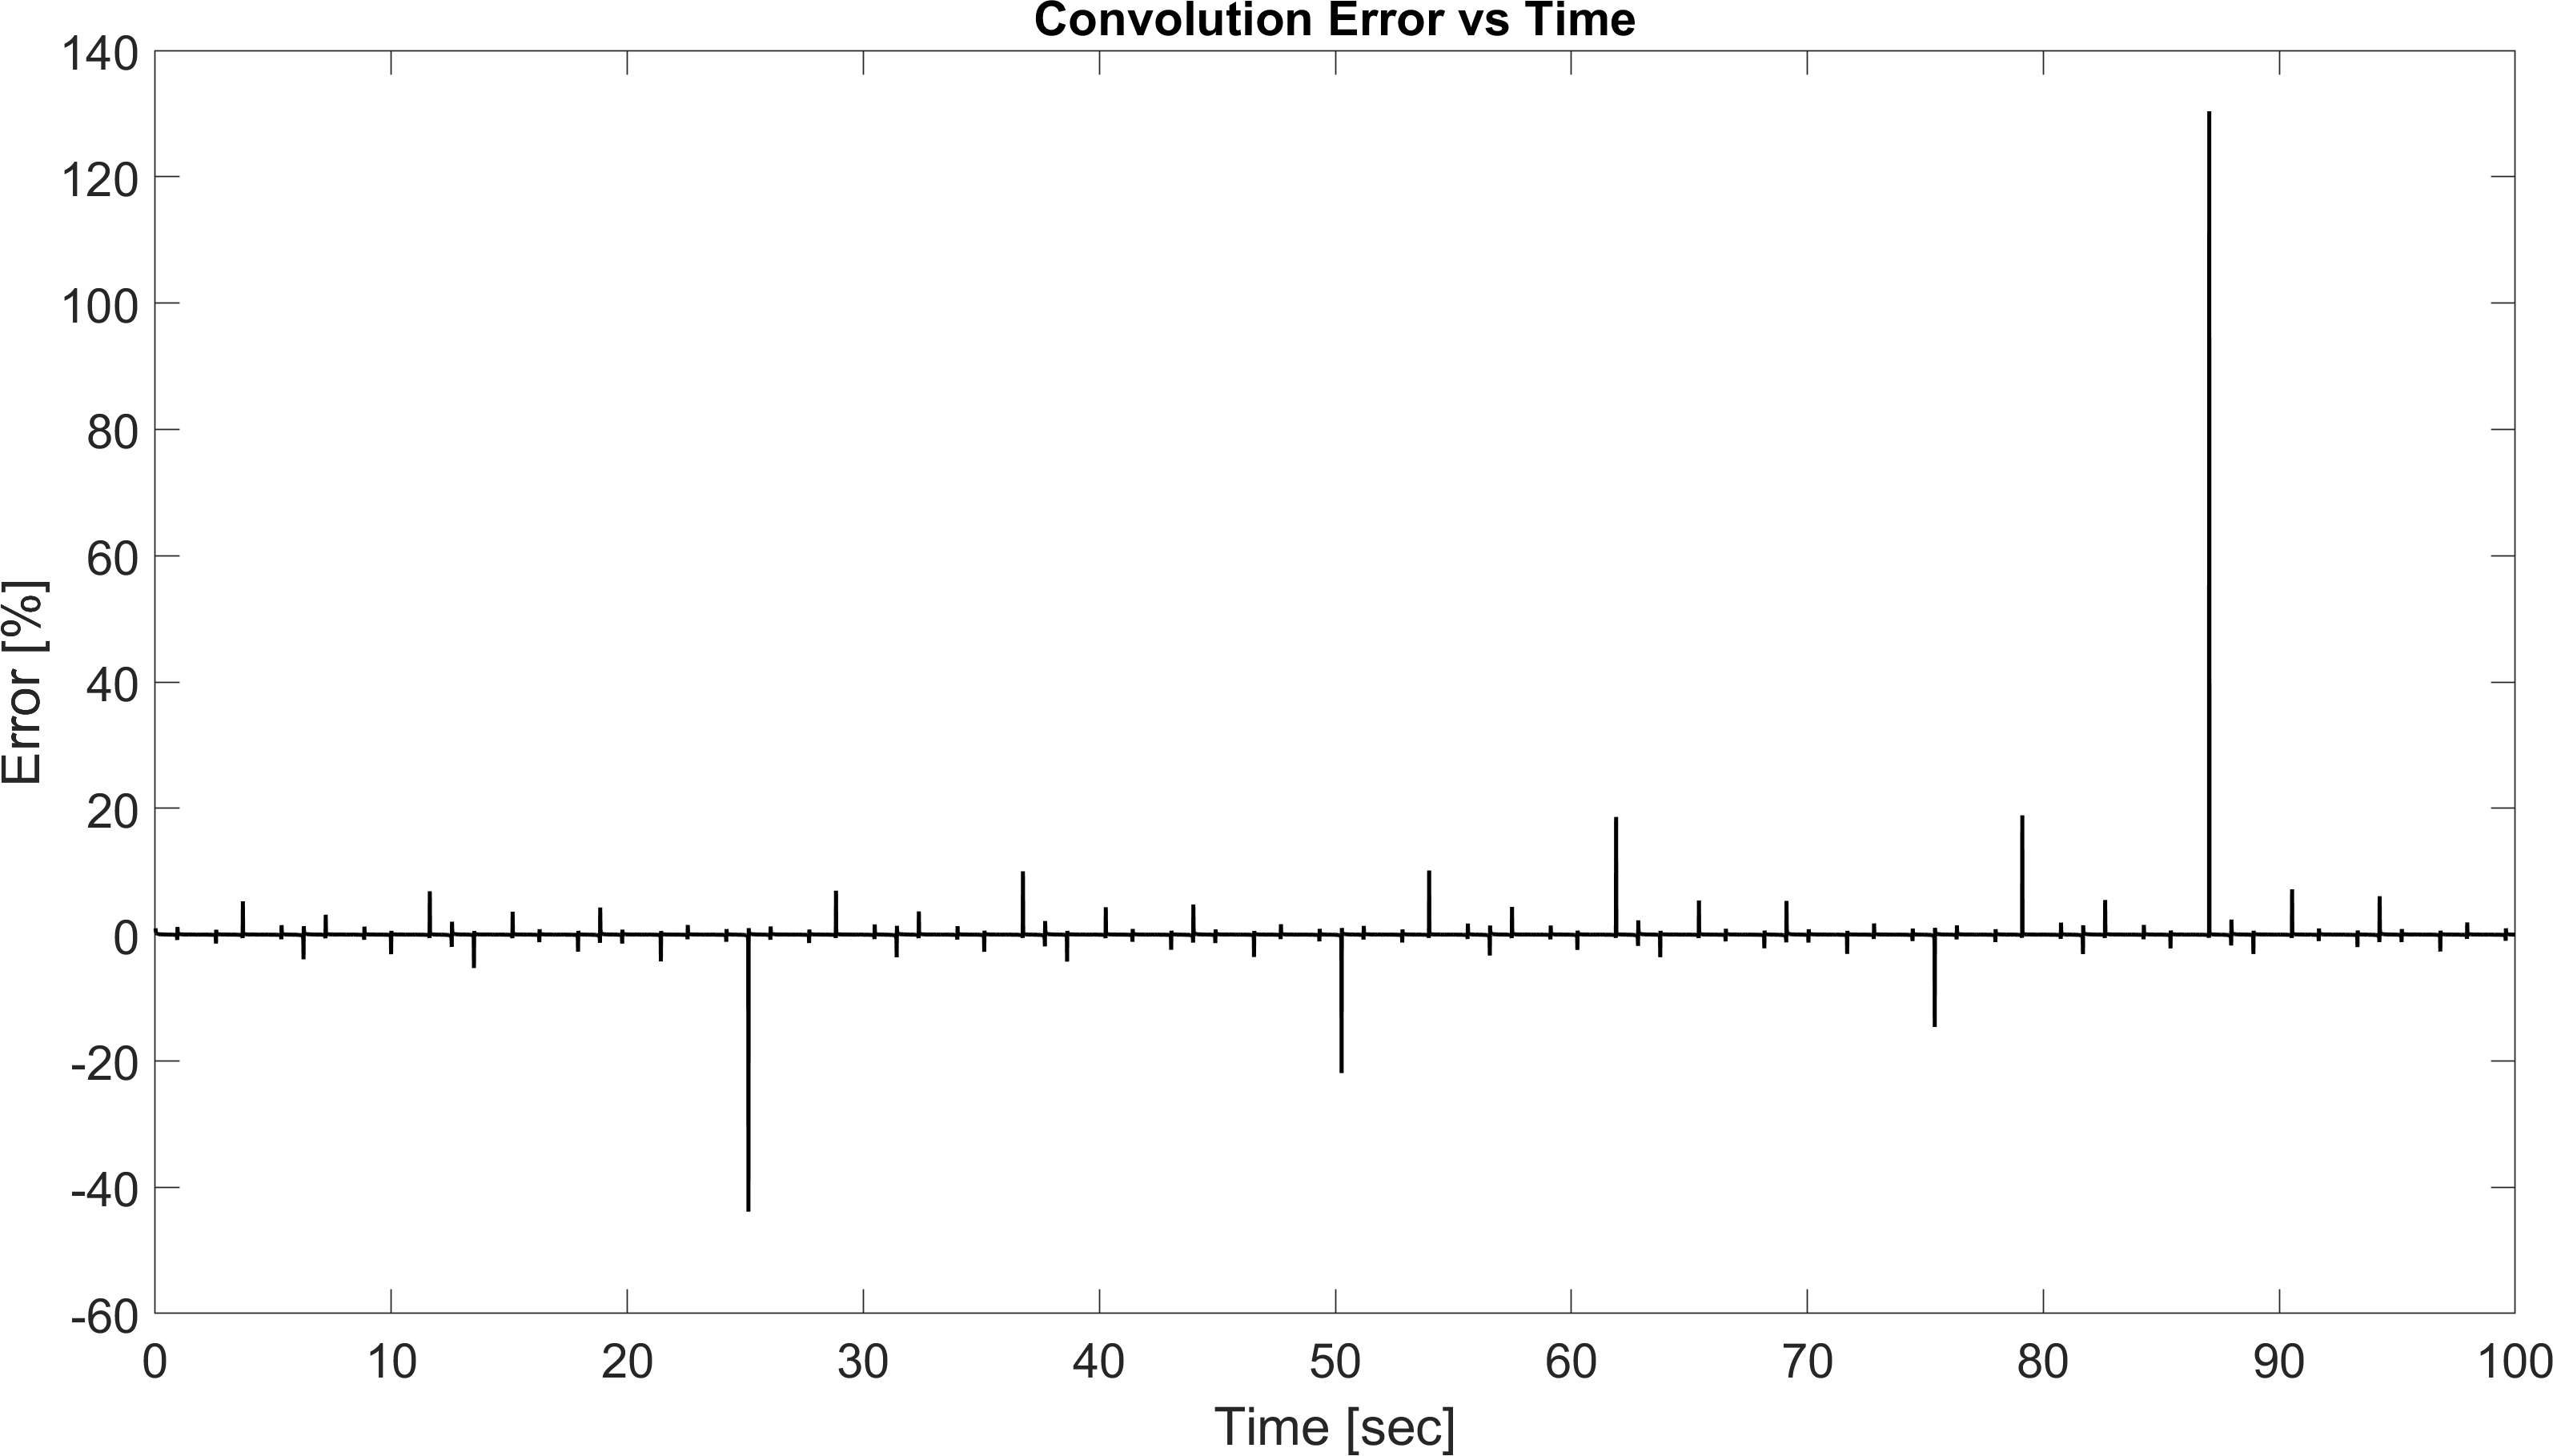
\includegraphics[width=1\textwidth,left]{MCHE 6390/Project 2/Figures/Figure_7.png}
    \captionsetup{justification=raggedright,singlelinecheck=false}
    \caption{Algorithm error}
    \label{fig:algerr}
\end{figure}
\noindent Note that although the error isn't perfect, it is generally very good, with the rms being only 1.46\%. Based off this, we can give good confidence that the solutions we obtained will be satisfactory.

\newpage
\section*{Appendix}
\subsection*{MCHE\_6390\_MDOF.m}
\begin{lstlisting}[style=Matlab-editor]
function [X,L,U] = MCHE_6390_MDOF(M,K,Z,F,B_f,IC_p,IC_v,t,Options)
%   MCHE_6390

% Ensure number of arguments is correct
narginchk(8,9);
nargoutchk(0,3);

% Convert string to character arrays
if nargin > 8
    Options = convertStringsToChars(Options);
else
    Options = 'NoOptions';
end

[Mn,~] = size(M);

% Validate attributes of inputs
validateattributes(F,{'function_handle'},{'real'});
validateattributes(M,{'single','double'},{'real','finite','square',...
    'nonnegative'});
validateattributes(K,{'single','double'},{'real','finite','square',...
    'size',[Mn,Mn]});
% validateattributes(Z,{'single','double'},{'real','finite','size',...
%    [Mn,1],'>=',0,'<=',1});
validateattributes(IC_p,{'single','double'},{'real','finite','size',...
    [Mn,1]});
validateattributes(IC_v,{'single','double'},{'real','finite','size',...
    [Mn,1]});
validateattributes(t,{'single','double'},{'real','finite','size',[1,NaN]});

test = F(t(end));
[testp,~] = size(test);

validateattributes(B_f,{'single','double'},{'binary','size',...
    [Mn,testp]});

% Solve generalized eigenvalue problem
[U_I,L_I] = eig(K,M);

% Select diagonal entries from L_I.^0.5 and sort them in increasing order
[L,I] = sort(diag(L_I.^0.5));

% Initialize U
U = zeros(length(M),length(M));

% Mass normalize U
for i = 1:length(M)
    U(:,i) = U_I(:,I(i))./sqrt((U_I(:,i)'*M*U_I(:,i)));
end

% Calculate Psi
Psi = U'*B_f;

% Calculate Modal Initial Conditions
r_0 = (U^-1)*IC_p;
r_0_dot = (U^-1)*IC_v;

% Calculate A and phi
A = sqrt((((r_0_dot+Z.*L.*r_0).^2)+((r_0.*L.*sqrt(1-Z.^2)).^2))./...
    ((L.*sqrt(1-Z.^2)).^2));
phi = atan2(L.*sqrt(1-Z.^2).*r_0,r_0_dot+Z.*L.*r_0);

% Initialize X_H
X_H = zeros(length(t),length(M));

for i = 1:length(t)
    X_H(i,:) = U*(A.*exp(-Z.*L*t(i)).*sin(L.*sqrt(1-Z.^2)*t(i)+phi));
end

X_P = U*Convolution(F,L,L.*sqrt(1-Z.^2),Z,t,Psi);

X = X_P'+X_H;

if isequal(Options,'Plot')
    figure(1)
    plot(t,X_H(:,1))
    
    figure(2)
    plot(t,X_P(1,:))
    
    figure(3)
    plot(t,X(:,1))
end

function C = Convolution(f,wn,wd,z,t,Psi)
% This is the old way of doing convolution. It is incredibly
%inefficient and with the new algorithm, I can do it many millions of
%times faster. 
%{
% Impulse response
g = @(t,tau,wn,wd,z) (1./wd).*exp(-z.*wn*(t-tau)).*sin(wd*(t-tau));

% Compute convolution, sum over p
C = sum(Psi.*(integral(@(tau) g(t,tau,wn,wd,z)*f(tau)',0,t,...
    'ArrayValued',true)),2);
%}

dt = t(2)-t(1);

% m-by-length(t)
gv = (1./wd).*exp(-z.*wn.*t).*sin(wd.*t);
[m,~] = size(gv);

% n-by-length(t)
fv = f(t);
[n,~] = size(fv);

C = zeros(m,n,length(t));

for j = 1:m
    Ly = length(gv(1,:))+length(fv(1,:))-1;
    Ly2 = pow2(nextpow2(Ly));

    D = zeros(m,n,Ly);

    for k = 1:n
        %D(j,k,:) = Psi(j,k)*ifft(fft(gv(j,:),Ly2).*fft(fv(k,:),Ly2),Ly2);
        D(j,k,:) = Psi(j,k)*conv(gv(j,:),fv(k,:));
        C(j,k,:) = D(j,k,1:length(t));
    end
end
C = sum(C,2);
C = dt*permute(C,[1,3,2]);

end
end
\end{lstlisting}
\subsection*{MCHE\_6390\_MDOF\_Test\_Case.m}
\begin{lstlisting}[style=Matlab-editor]
U = [1,3;2,-1];
M = (U^-1)'*eye(2)*(U^-1);
K = (U^-1)'*[4,0;0,9]*(U^-1);
% M = eye(2);
% K = [4,0;0,16];
Z = zeros(2,1);
F = @(t) 5+0*t;
B_f = [0;1];
IC_p = zeros(2,1);
IC_v = zeros(2,1);
t = linspace(0,100,10000);
Options = 'No_Plot';

[X,L,U] = MCHE_6390_MDOF(M,K,Z,F,B_f,IC_p,IC_v,t,Options);

err = (X(:,1)'-(+2.5-2.5*cos(2*t)-5/3+(5/3)*cos(3*t)))./...
    (2.5-2.5*cos(2*t)-5/3+(5/3)*cos(3*t));

plot(t,err)
\end{lstlisting}
\newpage
\subsection*{MCHE\_6390\_Project\_2.m}
\begin{lstlisting}[style=Matlab-editor]
lb = zeros(8,1);
ub = 1*ones(8,1);
options = optimoptions('fmincon','Display','iter',...
    'MaxFunctionEvaluations',4000,'TolCon',1e-7);

% Z = [0.318794341697629;0.121374568700831;0.00418762393140811;...
%    0.140885049913344;0.208792397688633;0.254387876321811;...
%    0.228947979430005;0.00868696814997558];
% Z = fmincon(@(z) fun3(z),Z,[],[],[],[],lb,ub,@(z)fun2(z),options);
Z = zeros(8,1);

[X,L,U,theta_rms,theta] = fun1(Z);

function [X,L,U,theta_rms,theta] = fun1(Z)
% Load in Data
load('MCHE_6390_Project_2_Load_Cases.mat','t','f1','f2')

% Masses
M_1 = 1.5;
M_2 = 1.5;
M_3 = 1.5;
M_4 = 0.2;
M_5 = 0.05;
M_6 = 0.04;
M_7 = 0.02;
M_8 = 0.03;

% Physical Parameters
E = 69*10^9;
r_o = 2.54*10^-2;
r_i = (2.54*10^-2)-(0.1*10^-2);
L_1 = 0.75;
L_2 = 0.75;
L_3 =  0.375;

% Calculate moment of inertia
I = 0.25*pi*(r_o^4-r_i^4);

% Stiffnesses;
K_1 = 10*10^3;
K_2 = 10*10^3;
K_3 = 50*10^3;
K_4 = 50*10^3;
K_5 = 50*10^3;
K_6 = 50*10^3;
K_7 = 48*E*I/(L_1^3);
K_8 = 48*E*I/(L_2^3);
K_9 = 48*E*I/(L_3^3);

% Assemble mass and stiffness matrices
K = [K_8+K_7+K_1+K_2,-K_8,0,-K_1-K_2,0,0,0,0;...
    -K_8,K_3+K_4+K_8+K_9,-K_9,0,-K_3,-K_4,0,0;...
    0,-K_9,K_5+K_6+K_9,0,0,0,-K_5,-K_6;...
    -K_1-K_2,0,0,K_1+K_2,0,0,0,0;...
    0,-K_3,0,0,K_3,0,0,0;...
    0,-K_4,0,0,0,K_4,0,0;...
    0,0,-K_5,0,0,0,K_5,0;...
    0,0,-K_6,0,0,0,0,K_6];
M = eye(8).*[M_1;M_2;M_3;M_4;M_5;M_6;M_7;M_8];

% Assumed Damping
Z = ones(8,1)*0.001+Z;

% Define function F through linear interpolation
F = @(T) [interp1(t,f1,T);interp1(t,f2,T)];

% Define B_f using given information
B_f = [1,1;0,1;0,1;0,1;0,1;0,1;0,1;0,1];

% zero initial conditions
IC_p = zeros(8,1);
IC_v = zeros(8,1);

% Plot?
Options = 'No_Plot';

% Use MDOF code
[X,L,U] = MCHE_6390_MDOF(M,K,Z,F,B_f,IC_p,IC_v,t,Options);

theta_1 = atan2d(X(:,5)-X(:,6),0.1);
theta_2 = atan2d(X(:,8)-X(:,7),0.1);

theta = theta_1-theta_2;
theta_rms = rms(theta_1-theta_2);
end
function [c,c_eq] = fun2(z)

c_eq = zeros(2,1);
% constraint given by problem
[X,~,~,theta_rms] = fun1(z);
c(1) = theta_rms-0.2;
c(2) = max(X(:,4))-2*10^-3;
 
end
function cost = fun3(z)
% Cost function
cost = 100000*sum((z-0.001).^2);
end
\end{lstlisting}
\newpage
\subsection*{MCHE\_6390\_Project\_2\_Figures.m}
\begin{lstlisting}[style=Matlab-editor]
% load('MCHE_6390_Project_2_Data.mat')
%{
figure(1)
% Plot
p1 = plot(t,X(:,4),'-k','LineWidth',1.5);
% limits
xlim([t(1) t(end)])
% ylim([-0.002 0.002])
% Title and axis labels
title('Response of Instrument 1 vs Time','FontSize',18)
xlabel('Time [sec]','FontSize',18)
ylabel('Displacement [m]','FontSize',18)
ax = gca;
% Set x and y font sizes.
ax.XAxis.FontSize = 18;
ax.YAxis.FontSize = 18;
% Create and format legend
%legend([p1], 'Compressor Inlet Pressure [PSIA]',...
%    'Compressor Outlet Pressure [PSIA]','location', 'SouthOutside',...
%    'FontSize',18)
%set(legend, 'box', 'off')
% Make plot size of computer screen
set(gcf, 'Units', 'Normalized', 'OuterPosition', [0 0 1 1]);
% Set background color to white
set(gcf, 'Color', 'w');
export_fig Figure_1.png -m2.5

figure(2)
% Plot
p1 = plot(t,theta,'-k','LineWidth',1.5);
% limits
xlim([t(1) t(end)])
%ylim([-0.002 0.002])
% Title and axis labels
title('\theta_{1}-\theta_{2} vs Time','FontSize',18)
xlabel('Time [sec]','FontSize',18)
ylabel('Angular Displacement [deg]','FontSize',18)
ax = gca;
% Set x and y font sizes.
ax.XAxis.FontSize = 18;
ax.YAxis.FontSize = 18;
% Create and format legend
%legend([p1], 'Compressor Inlet Pressure [PSIA]',...
%    'Compressor Outlet Pressure [PSIA]','location', 'SouthOutside',...
%    'FontSize',18)
%set(legend, 'box', 'off')
% Make plot size of computer screen
set(gcf, 'Units', 'Normalized', 'OuterPosition', [0 0 1 1]);
% Set background color to white
set(gcf, 'Color', 'w');
export_fig Figure_2.png -m2.5
%}
figure(3)
% Plot
p1 = plot(t,err,'-k','LineWidth',1.5);
% limits
xlim([t(1) t(end)])
%ylim([-0.002 0.002])
% Title and axis labels
title('Convolution Error vs Time','FontSize',18)
xlabel('Time [sec]','FontSize',18)
ylabel('Error [%]','FontSize',18)
ax = gca;
% Set x and y font sizes.
ax.XAxis.FontSize = 18;
ax.YAxis.FontSize = 18;
% Create and format legend
%legend([p1], 'Compressor Inlet Pressure [PSIA]',...
%    'Compressor Outlet Pressure [PSIA]','location', 'SouthOutside',...
%    'FontSize',18)
%set(legend, 'box', 'off')
% Make plot size of computer screen
set(gcf, 'Units', 'Normalized', 'OuterPosition', [0 0 1 1]);
% Set background color to white
set(gcf, 'Color', 'w');
export_fig Figure_7.png -m2.5
\end{lstlisting}
\end{document}